\documentclass[a4paper,10pt]{article}
\usepackage[ngerman]{babel}
\usepackage[utf8]{inputenc}
\usepackage[a4paper,vmargin={20mm,20mm},hmargin={20mm,10mm}]{geometry}
\usepackage[T1]{fontenc}

\usepackage{tocloft, multicol} 
\usepackage{amsmath, amsfonts, amssymb} 
\usepackage{booktabs} 
\usepackage{bm}  
\usepackage{caption}
\usepackage{subcaption}
\usepackage{enumitem}
\usepackage{graphicx} 
\usepackage{listings}
\usepackage{mathtools}
\usepackage[dvipsnames]{xcolor}
\usepackage{wrapfig,lipsum,threeparttable}
\usepackage{footmisc, fixfoot}



\DeclareFixedFootnote{\fnrefa}{ P. T. Boggs and J. E. Rogers, “Orthogonal Distance Regression,” in “Statistical analysis of measurement error models and applications: proceedings of the AMS-IMS-SIAM joint summer research conference held June 10-16, 1989,” Contemporary Mathematics, vol. 112, pg. 186, 1990. }
\DeclareFixedFootnote{\fnrefb}{ Dr. J.Wagner - Physikalisches Anfängerpraktikum - V. 1.1 Stand 1/2018, Versuch 223}


\lstset{literate=%
    {Ö}{{\"O}}1
    {Ä}{{\"A}}1
    {Ü}{{\"U}}1
    {ß}{{\ss}}1
    {ü}{{\"u}}1
    {ä}{{\"a}}1
    {ö}{{\"o}}1
    {~}{{\textasciitilde}}1
}
\lstset{%
backgroundcolor=\color{gray!32},
basicstyle=\ttfamily\footnotesize,
numbers=left,numberstyle=\scriptsize,
frame=single,
breaklines=true,
}

\usepackage[wby]{callouts}
\title{WS19/20, PAP2.1, Versuch 223:\\Brown'sche Bewegung}
\date{Versuchsdurchführung: \\12. November, 2019}
\author{Praktikanten:\\Gerasimov, V. \& Reiter, L.\\\\ Betreuer:\\ Schmidt-Kaler, F.}


\begin{document}
\maketitle

\newpage

\tableofcontents

\addtocontents{toc}{~\hfill\textbf{Seite}\par}


\section{Einführung}\boldmath
In diesem Versuch\fnrefb werden wir die Brown'sche Bewegung von Partikeln suspensiert in Wasser mit einem Mikroskop beobachten und deren statistische Bewegung untersuchen. Durch Vermessen der Teilchenbahn und der Berechnung der pro Zeiteinheit auftretenden mittleren Verschiebung, können
wir die Boltzmannkonstante \(k_B\) bestimmen. Eine genaue Bestimmung der Boltzmannkonstante mit Hilfe der Brownschen Bewegung ist nur bei der Beobachtung sehr vieler Einzelschritte möglich und daher im Praktikum aus Zeitgründen nicht möglich. Bei einer sorgfältigen
Durchführung ist aber eine Genauigkeit von besser als 10 \% möglich.
\section{Versuchsaufbau, Literaturwerte \& Vorbereitung}
\begin{itemize}
\item Durchlichtmikroskop Motic B1 mit CCD-Kamera
\item Kugelförmige Partikel suspendiert in Wasser
\item Thermometer
\item Objektmikrometer
\item Boltzmann-Konstante\footnote{https://physics.nist.gov/cgi-bin/cuu/Value?k, [Stand 17.1.2019]} \(k_B=1.380649\times 10^{-23}\:J\:K^{-1}\) ist als fundamentale Konstante exakt festgelegt und hat besitzt deswegen Unsicherheit.
\end{itemize}

\pagebreak
\section[Durchführung]{Durchführung\fnrefb}
 \begin{wrapfigure}{r}{0.45\textwidth}
  \centering
  \begin{annotate}{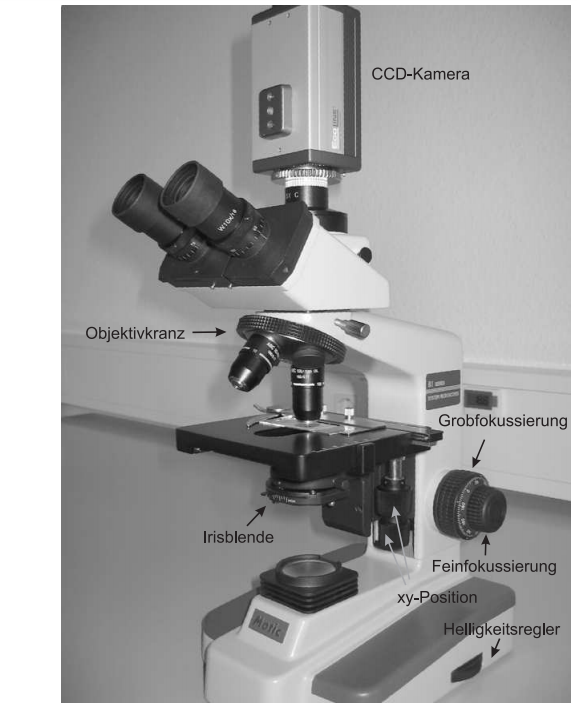
\includegraphics[width=0.5\textwidth]{aufbau2.png}}{1}
  \end{annotate}
    \caption{Mikroskop}
 \label{fig:aufbau2}
\end{wrapfigure} 
\subsection{Probenpräparation} Wir wollen die Brown'sche Bewegung suspendierter Latex-Partikel in Wasser untersuchen. 
 Um diese mit dem Mikroskop beobachten zu können, benötigen wir eine Probenfassung, die einerseits dick genug ist, so dass sich die suspendierten Partikel darin frei bewegen können, andererseits muss diese auch dünn genug sein, damit eine Fokussierung mit dem Mikroskop möglich ist. Um dies zu gewährleisten, werden wir zunächst eine Probenfassung gemäß Abbildung \ref{fig:aufbau1} anfertigen: Auf einen Objektträger wird ein doppelseitiges Klebeband aufgebracht, in dessen Mitte zuvor ein Loch ausgestanzt wurde. In diese Öffnung wird die Probenflüssigkeit eingefüllt und mit einem Deckglas verschlossen. Das doppelseitige Klebeband erfüllt dabei zwei Aufgaben: Zum einen vergrößert dieses das Probenvolumen, so dass sich die suspendierten Partikel frei bewegen können, zum anderen dient es zur Abdichtung der Flüssigkeit, wodurch ungewollte Strömungen durch Verdunstungsprozesse unterdrückt werden.\\\\
Wir fertigen vor Versuchsbeginn stets eine neue Probe an, schneiden dazu ein Stück doppelseitiges Klebeband passend auf die Größe des Deckglases (\(24\: mm \times 32\: mm l\)) zurecht und stanzen danach mit dem Locheisen zentrisch ein Loch in das Klebeband (mit Holzunterlage). 
Anschließend kleben wir das Klebeband mittig auf den Objektträger und entfernen die Abdeckfolie. Wir Wir schütteln die Flasche mit der Probenflüssigkeit gut durch und pipettieren \(250\:\mu l\) der Probenflüssigkeit in die ausgestanzte Öffnung des Klebebands. Wir Werfen die Pipettenspitze nach Gebrauch sofort in den Abfall. Der Durchmesser der Partikel ist auf der Flasche angegeben.
Wir notieren diesen Wert, legen das Deckglas auf das doppelseitige Klebeband und drucken es mit einem Papiertuch vorsichtig an. Dabei darf ruhig etwas von der Flüssigkeit herausfließen. Allerdings dürfen sich keine (größeren) Luftblasen in der Flüssigkeit bilden! Danach trocknen die Probe mit einem Papiertuch ab und und geben auf die Mitte des Deckglases einen Tropfen Immersionsöl. Wir spannen nun die Probe auf den Mikroskoptisch (Abbildung \ref{fig:aufbau2}) ein und  wählen am Objektivkranz des Mikroskops das Objektiv mit 100-facher Vergrößerung und einer Numerische Apertur NA=1.25 aus (100/1.25 ).
\begin{figure}[htb]
  \centering
  \begin{annotate}{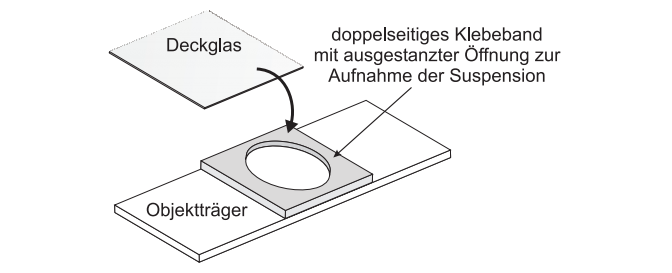
\includegraphics[width=0.5\textwidth]{aufbau1.png}}{1}
  \end{annotate}
\caption{Skizze der Probenfassung. Die ausgestanzte Öffnung des doppelseitigen Klebebands wird mit der zu untersuchenden Suspension befüllt und anschließend mit dem Deckglas verschlossen.}
\label{fig:aufbau1}
\end{figure}

\subsection{Aufnahme einer Bildfolge}
Wir starten vom Desktop aus das Programm \texttt{Kamera.exe}. Dieses Programm nimmt in einem festen Zeitabstand
ein Bild auf und speichert dieses auf dem Computer. Wir tragen im Messprogramm für den Zeitabstand \(1\:s\) ein und schalten die Option \glqq Bilder speichern\grqq~zunächst ab und 
suchen uns ein Partikel aus, in dessen unmittelbarer Umgebung sich keine anderen Partikel befinden und stellen die xy-Position des
Mikroskoptisches so ein, dass sich das ausgewählte Partikel im Zentrum des Mikroskopbildes befindet. Zur Verbesserung des Kontrastes sollten wir die Irisblende am Kondensor auf die Position MIN stellen. Da die Brown'sche Bewegung nicht nur in der xy-Bildebene, sondern auch in z-Richtung erfolgt, wird es passieren, dass das zu beobachtende Partikel
aus dem Fokus läuft und somit nicht mehr sichtbar wird. Um dem entgegenzuwirken, muss man die Fokussierung des Mikroskops mit dem Feinregler dauernd nachjustieren. Dies erfordert einiges an Feingefühl und besonders Konzentration.
Wir führen zunächst eine Probemessung durch: Damit sich die Probe
durch die Mikroskopbeleuchtung nicht zusätzlich aufheizt, drehen die
Helligkeit auf das Minimum zurück. Die Kamera ist auch bei dieser Minimalbeleuchtung empfindlich genug, kontrastreiche Bilder zu liefern. Das Programm wird durch Anklicken des Pfeils in der linken oberen Ecke gestartet und wir versuchen der Bewegung eines Partikels über mehrere Minuten auf dem Monitor zu folgen. Sobald das Partikel auch nur leicht unscharf
zu erkennen ist, müssen wir sofort mit dem Feintrieb des Mikroskops den Fokus vorsichtig nachstellen. Das Partikel muss während der ganzen Zeit eindeutig erkennbar sein! Wenn wir nun genug Übung im Nachfokussieren erlangt haben und die zuvor genannten Punkte bezüglich der systematischen Fehler berücksichtigt haben, können wir mit der eigentlichen Messung beginnen. Wir stoppen das
Messprogramm. Wir schalten die Option \glqq Bilder speichern\grqq~ein und starten
wir erneut das Programm. Insgesamt ist jede Sekunde und mindestens \(150\:mal\), ein Bild aufzunehmen. Nach der Messung entfernen wir die Probe und werfen diese in den Abfall.
\subsection{Temperatur} 
Wir notieren die Zimmertemperatur \(T\) im Versuchsraum mit Hilfe des Thermometers.\\
Messung wurden dem Versuchsprotokoll (12. Novemberr, 2019) entnommen und nach hier übertragen:
\begin{align*}
T&=22.6(7)\:^{\circ}C
\end{align*}
\subsection{Eichung des Abbildungsmaßstabs} 
Um später die Position des Partikels ausmessen zu können, müssen wir den Abbildungsmaßstab des Mikroskops bestimmen und benutzen dazu das ausliegende Objektmikrometer. Wir geben einen Tropfen Immersionsöl auf das Objektmikrometer und legen dieses auf den Mikroskoptisch. Wir stellen vorsichtig den Fokus ein und positionieren den Mikroskoptisch so, dass man den Maßstab erkennen kann. Wir beenden das Messprogramm und starte das Programm \texttt{Eichung.exe}, optimieren nochmals die Bildschärfe und speichern dann das Eichbild(Abb.\ref{fig:eich}) ab. Wir reinigen das Objektmikrometer mit einem Papiertuch und legen es zurück in die Aufbewahrungsbox.
Messung wurden dem Versuchsprotokoll (12. Novemberr, 2019) entnommen und nach hier übertragen:
\begin{align*}
 \text{Anzahl der Pixel pro }\quad{20\:\mu m}: \quad 222\pm 3
\end{align*}
\begin{figure}[htb]
  \centering
  \begin{annotate}{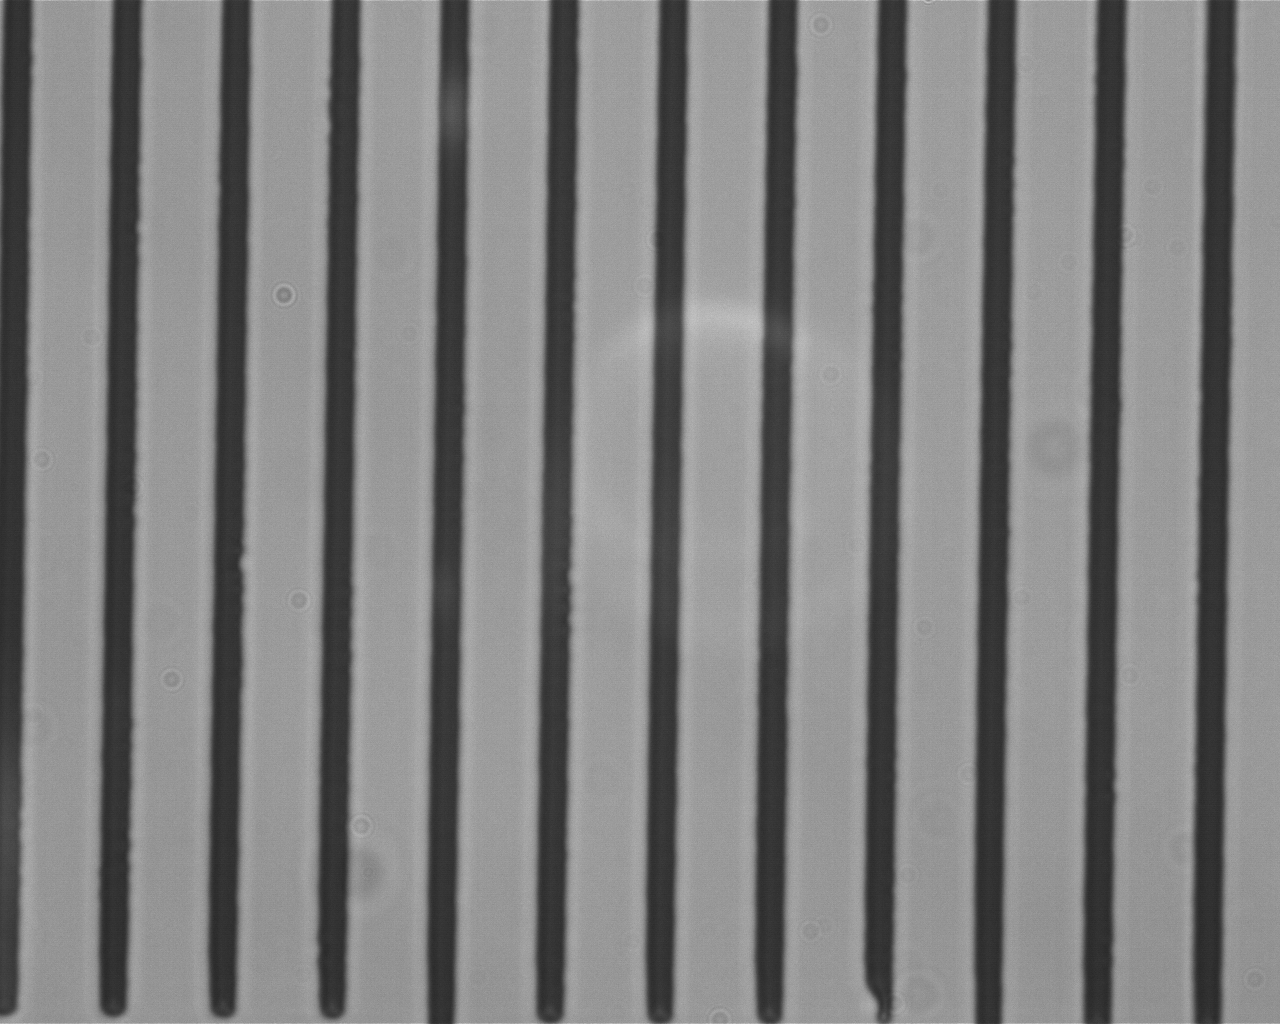
\includegraphics[width=0.5\textwidth]{eich.png}}{1}
  \end{annotate}
\caption{Eichbild}
\label{fig:eich}
\end{figure}

\begin{figure}[htb]
  \centering
  \begin{annotate}{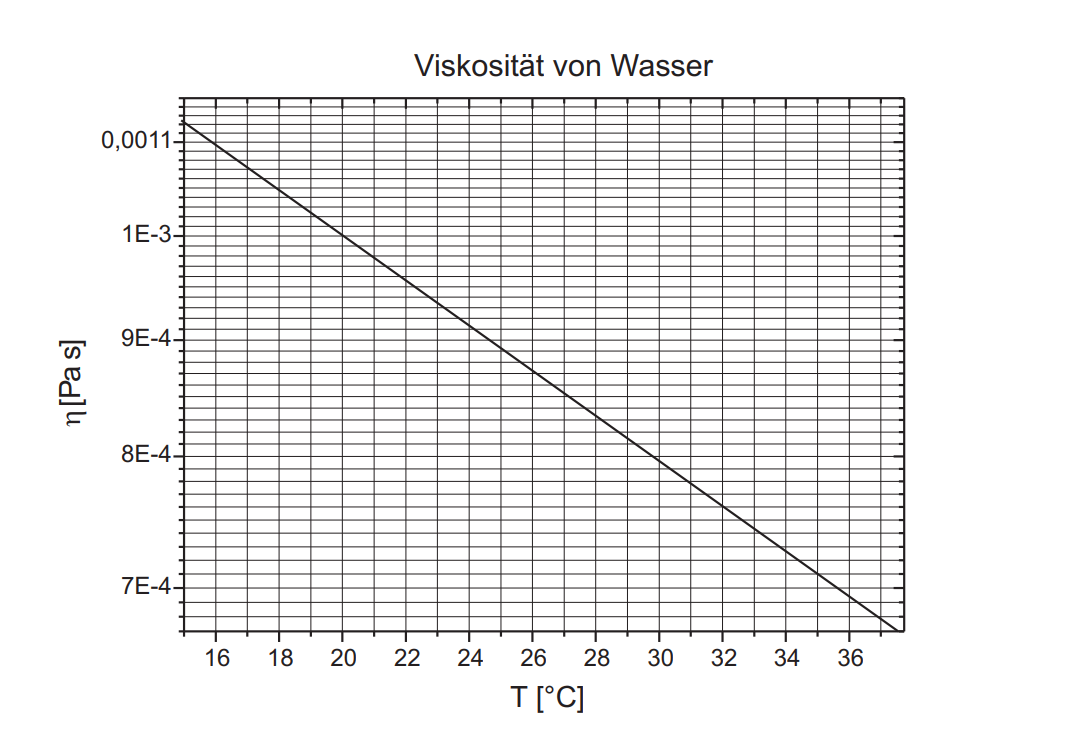
\includegraphics[width=0.8\textwidth]{pic1.png}}{1}
  \end{annotate}
\caption{}
\label{fig:pic1}
\end{figure}

\section{Kurvenanpassung mit Python}
\subsection{Source Code \& Input}
Für eine der folgenden Rechnungen gehen davon aus, dass die Kumulative Verschiebung linear mit der Zeit zunimmt.
Daher ist unser funktionales Modell für die Ausgleichungsrechnung wie folgt:
\begin{equation} \label{eq:Fit1}
	\boxed{\langle r^2 \rangle = \langle \Delta t \rangle S + b}
\end{equation} 
So sieht unsere Python-Implementierung aus:\\

Header:
\begin{lstlisting}
%matplotlib inline
import matplotlib.pyplot as plt
import numpy as np
from scipy.stats import norm
from decimal import Decimal

def format_e(n):
    a = '%e' % Decimal(n)
    return a.split('e')[0].rstrip('0').rstrip('.')+'e'+a.split('e')[1]

def comma_to_float(valstr):
    return float(valstr.decode('utf-8').replace(',','.'))

\end{lstlisting}

Messwerte aus DAT-Datei in den Einheiten [s],[\(\mu m\)] und [\(\mu m\)]:\begin{lstlisting}
t, x, y = np.loadtxt('data\Messung2.dat', skiprows=1, usecols=(1, 2, 3), converters= {1: comma_to_float, 2:comma_to_float, 3:comma_to_float}, unpack=True)

\end{lstlisting}

Diagramm (Abb.\ref{fig:Fig1}) wird erstellt:\begin{lstlisting}
fig, ax = plt.subplots(1, figsize=[6.4, 4.8])
plt.plot(x, y, lw=1, color='C3', marker='s', alpha=.50, label='Messdaten')
plt.title('Brownsche Bewegung')
plt.xlabel('Position '+r'${x}$'+' '+r'${[{\mu}m]}$')
plt.ylabel('Position '+r'${y}$' + ' '+r'${[{\mu}m]}$')
plt.legend(loc='best')

fig.savefig('figures/223_Fig1.pdf', format='pdf', bbox_inches='tight')

\end{lstlisting}
Abgeschätzter Kugelradius \(a\) des betrachteten Teilchens wurde durch nachträgliche Betrachtung der aufgenommenen Bilder in Pixeln bestimmt  und danach mit Hilfe der Eichungsdaten 
\[a= (8\pm2)px = (8\pm2)px \frac{20\:\mu m}{222\: px}\]
auf \(\mu m\) umgerechnet: \begin{lstlisting}
a = 8 * (20/222)
a_std = 2 * (20/222)

\end{lstlisting}

Zimmertemperatur \(T\) wie zuvor gemessen: \begin{lstlisting}
T = 22.6 + 273.15 
T_std = 0.7

\end{lstlisting}

Viskosität \(\eta=9.4(2)\times10^{-4}\:Pa\:s\) von Wasser in uns gegebener Abbildung \ref{fig:pic1} für \(T =22.6(7)\:^{\circ}C\) abgelesen: \begin{lstlisting}
eta = 9.4e-4
eta_std = 0.2e-4

dt = np.array([])
dx = np.array([])
dy = np.array([])
i = 0
while i < t.size-1:
    dt = np.append(dt,t[i+1]-t[i])
    dx = np.append(dx,x[i+1]-x[i])
    dy = np.append(dy,y[i+1]-y[i])
    i = i+1
r_squared = dx**2+dy**2

r_squared_mean = np.mean(r_squared)
r_squared_mean_std = np.std(r_squared)/np.sqrt(r_squared.size)
dt_mean = np.mean(dt)
dt_mean_std = np.std(dt)/np.sqrt(dt.size)

all_data = np.append(dx,dy)

counts = all_data.size
mu = np.mean(all_data)
sigma = np.std(all_data)

\end{lstlisting}

Plot-Umgebung wird angegeben:\begin{lstlisting}
x_fit = np.linspace(-4,4, 1000)
binwidth = sigma/2
x_bin = np.linspace((min(all_data))-binwidth/2, max(all_data)+binwidth/2, int((max(all_data)-min(all_data))/binwidth+1))
gauss = norm.pdf(x_fit, mu ,sigma)*counts*binwidth

\end{lstlisting}

Diagramm (Abb.\ref{fig:Fig2}) wird erstellt:\begin{lstlisting}
fig, ax = plt.subplots(1, figsize=[6.4 *1.5, 4.8])
plt.title('Histogramm der Verschiebungen')
plt.xlabel('Bewegung entlang 1 Dimension '+r'${{\Delta}x}$'+' bzw. '+r'${{\Delta}y}$'+' '+r'${[{\mu}m]}$')
plt.ylabel('counts')
plt.hist(all_data, bins=x_bin, color='C0', label='Histogram der Messdaten')
plt.plot(x_fit, gauss, 'C3-', lw=2, label='Gauß-Verteilung:\n'+r'${\mu}$'+' = '+str(format_plt(mu))+',\n'+r'${\sigma}$'+' = '+str(format_plt(sigma)))
plt.grid(True)
plt.legend(loc='best')

fig.savefig('figures/223_Fig2.pdf', format='pdf', bbox_inches='tight')



r_kumm = np.cumsum(r_squared)

\end{lstlisting}

darzustellende Daten werden übergeben:\begin{lstlisting}
x = t[:-1]
y = r_kumm

\end{lstlisting}

Fitfunktion \eqref{eq:Fit1} wird deklariert:\begin{lstlisting}
from scipy.optimize import curve_fit

def fit_func(x,a,b):
    return a*x+b

popt, pcov = curve_fit(fit_func, x, y)

\end{lstlisting}

Angabe welche Sigma-Umgebung der Fitfunktion im Diagramm dargestellt werden soll:\begin{lstlisting}
nstd = 8 
popt_top = popt+nstd*np.diag(pcov)
popt_bot = popt-nstd*np.diag(pcov)

\end{lstlisting}

Plot-Umgebung wird angegeben:\begin{lstlisting}
x_fit = np.linspace(min(x)-(max(x)-min(x))/10, max(x)+(max(x)-min(x))/10, 1000)
fit = fit_func(x_fit, *popt)
fit_top = fit_func(x_fit, *popt_top)
fit_bot = fit_func(x_fit, *popt_bot)

\end{lstlisting}

Diagramm (Abb.\ref{fig:Fig3}) wird erstellt:\begin{lstlisting}
fig, ax = plt.subplots(1, figsize=[6.4*2, 4.8*2])
plt.title('Kumulative Verschiebung')
plt.grid(True)
plt.plot(t[:-1], r_kumm, color='C3', marker='.', linewidth=0, label='Messdaten')
plt.plot(x_fit, fit, 'k', lw=1, label='Fit')
ax.fill_between(x_fit, fit_top, fit_bot, color='C3', alpha=.25, label=str(nstd)+r'$\sigma$'+'-Umgebung')
plt.xlabel('Zeit t [s]')
plt.ylabel('Summe $\Sigma (r_i^2)$ [${\mu m}^2$]')
plt.legend(loc='best')

fig.savefig('figures/223_Fig3.pdf', format='pdf', bbox_inches='tight')

\end{lstlisting}

Auslesen der Messergebnisse und Umwandlung der Abhängigkeit von Zeit zur Abhängigkeit vom Weg:\begin{lstlisting}
s = popt[0]
s_std = pcov[0][0]

\end{lstlisting}

Wir wollen die Boltzmann-Konstante \(k_{B}\) auf zwei verschiedene Weisen berechnen. Zuerst durch die Annahme, dass die verstrichene Zeit und das durchschnittliches Quadrat der Verschiebung proportional zusammenhängen, also: 
\begin{equation} \label{eq:k_B1}
	k_{B,1} = \frac{6 \pi  \langle r^2 \rangle a \eta}{4 T \langle \Delta t \rangle}
\end{equation} 
\begin{equation} \label{eq:Deltak_B1}
	\Delta k_{B,1} = k_{B,1} \sqrt{{\left(\frac{\Delta \langle r^2 \rangle}{\langle r^2 \rangle}\right)}^2+{\left(\frac{\Delta a}{a}\right)}^2+{\left(\frac{\Delta T}{T}\right)}^2+{\left(\frac{\Delta \langle \Delta t \rangle}{\langle \Delta t \rangle}\right)}^2}
\end{equation} 

Berechnung von \(k_{B,1}\) und \(\Delta k_{B,1}\) nach \eqref{eq:k_B1} bzw. \eqref{eq:Deltak_B1}:\begin{lstlisting}
k_1 = 6*r_squared_mean*np.pi*a/(4*T*dt_mean) * 1e-18 * eta
k_1_std = k_1*np.sqrt((r_squared_mean_std/r_squared_mean)**2+(a_std/a)**2+(T_std/T)**2+(dt_mean_std/dt_mean)**2+(eta_std/eta)**2)

\end{lstlisting}

Und danach durch Bestimmung der Steigung \(S\) einer Regressionslinie die die verstrichene Zeit auf kumulative Verschiebung abbildet (Abb.\ref{fig:Fig3}):
\begin{equation} \label{eq:k_B2}
	k_{B,2} = S \frac{6 \pi a \eta}{4 T}
\end{equation} 
\begin{equation} \label{eq:Deltak_B2}
	\Delta k_{B,2} = k_{B,2} \sqrt{{\left(\frac{\Delta S}{S}\right)}^2+{\left(\frac{\Delta a}{a}\right)}^2+{\left(\frac{\Delta T}{T}\right)}^2}
\end{equation} 

Berechnung von \(k_{B,2}\) und \(\Delta k_{B,2}\) nach \eqref{eq:k_B2} bzw. \eqref{eq:Deltak_B2}:\begin{lstlisting}
k_2 = 6*s*np.pi*a/(4*T) * 1e-18 * 9.4e-4
k_2_std = k_2*np.sqrt((s_std/s)**2+(a_std/a)**2+(T_std/T)**2++(eta_std/eta)**2)

\end{lstlisting}

Ausgabe der Messergebnisse wird erstellt:\begin{lstlisting}

print('Anzahl der Messungen = ', counts)
print('r_squared_mean [{\mu m}^2] = ', format_e(r_squared_mean), ' +- ', format_e(r_squared_mean_std))
print('dt_mean [s] = ', format_e(dt_mean))
print('Steigung:')
print('S [{\mu m}^2 / s] =', format_e(s), ' +- ', format_e(s_std))
print('Boltzmann-Konstante')
print('k_1 [J/K]: '+format_e(k_1)+' +- '+format_e(k_1_std))
print('k_2 [J/K]: '+format_e(k_2)+' +- '+format_e(k_2_std))
\end{lstlisting}


\subsection{Output}
\begin{lstlisting}
Anzahl der Messungen =  292
r_squared_mean [{\mu m}^2] =  1.574166e+00  +-  1.087616e-01
dt_mean [s] =  1.000473e+00

Steigung:
S [{\mu m}^2 / s] = 1.559976e+00  +-  3.188454e-05

Boltzmann-Konstante
k_1 [J/K]: 1.698465e-23 +- 4.420316e-24
k_2 [J/K]: 1.68395e-23 +- 4.225282e-24

\end{lstlisting}
Wir erfahren also dass,
\begin{align*}
\text{Anzahl der Messungen 1-dimensionaler Verschiebungen}: \quad & 292\\
\langle r^2 \rangle  =  &1.57(11)\:{\mu m}^2\\
\langle \Delta t \rangle  =  &1.000473\:s\\
 S  =  &1.559976(32) \:{\mu m}^2\:s^{-1}\\
 k_{B,1} = &1.70(44)\times10^{-23}\:J\:K^{-1}\\
 k_{B,2} = &1.69(42)\times10^{-23}\:J\:K^{-1}
\end{align*}
\begin{itemize}
\item Abbildung \ref{fig:Fig1} zeigt uns die Bewegung des beobachteten Teilchens während der gesamten Zeitspanne an.
\item Abbildung \ref{fig:Fig2} zeigt ein Histogramm der einzelnen Verschiebungen des Teilchens entlang der x- und y-Achse.
\item Abbildung \ref{fig:Fig3} zeigt uns kumulative Verschiebung des Teilchens an, also die genäherte Pfadlänge als Funktion der verstrichenen Zeit an.
\end{itemize}
\begin{figure}[htb]
  \centering
  \begin{annotate}{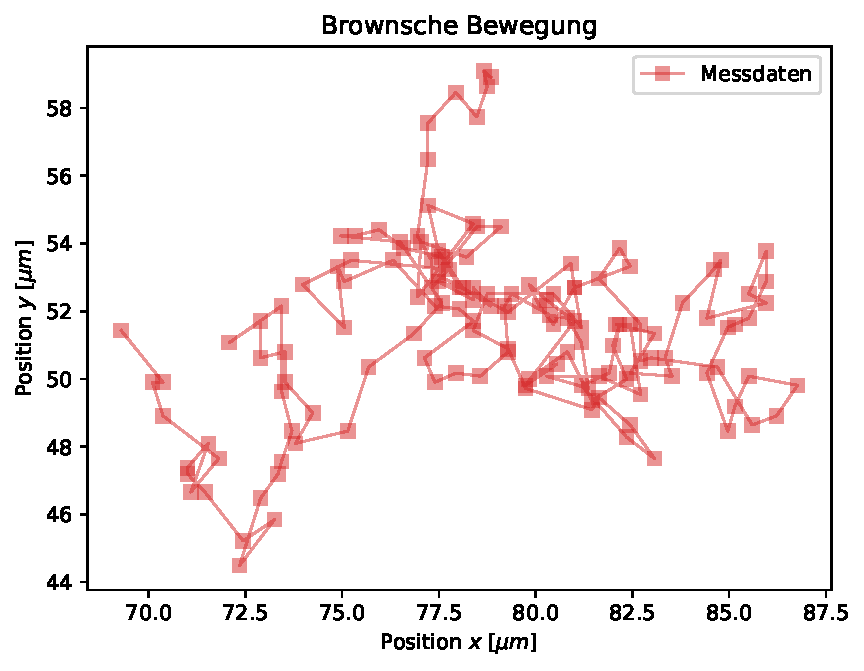
\includegraphics[width=0.8\textwidth]{223_Fig1.pdf}}{1}
  \end{annotate}
\caption{}
\label{fig:Fig1}
\end{figure}

\begin{figure}[htb]
  \centering
  \begin{annotate}{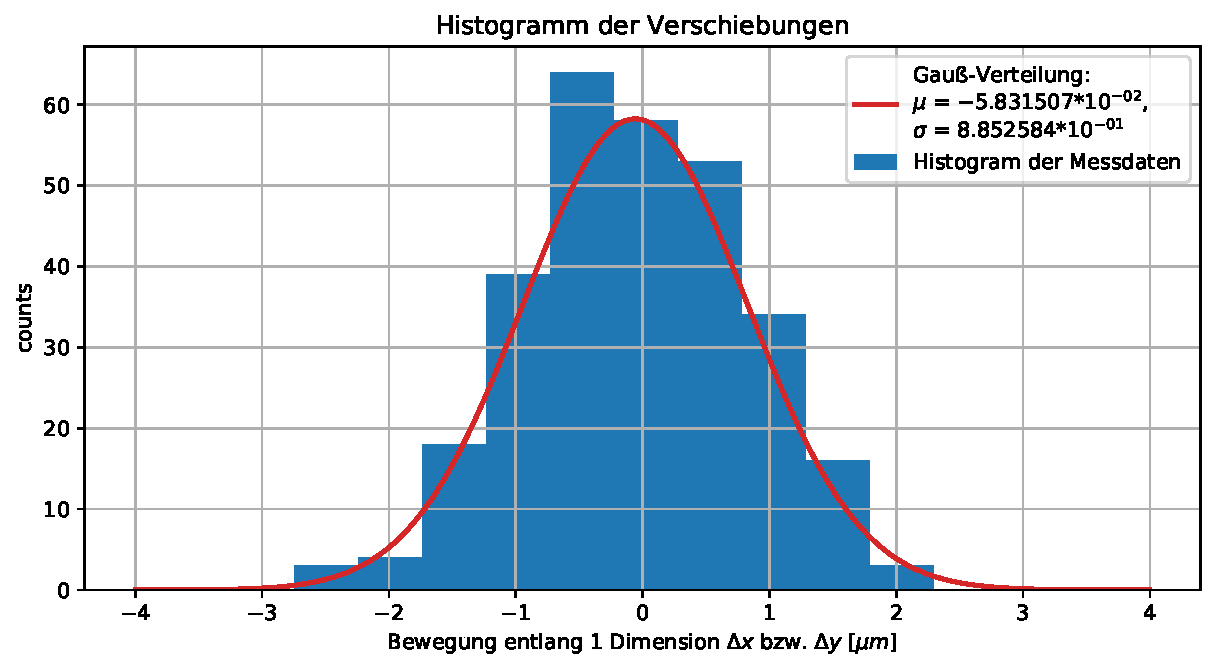
\includegraphics[width=0.8\textwidth]{223_Fig2.pdf}}{1}
  \end{annotate}
\caption{}
\label{fig:Fig2}
\end{figure}
\begin{figure}[htb]
  \centering
  \begin{annotate}{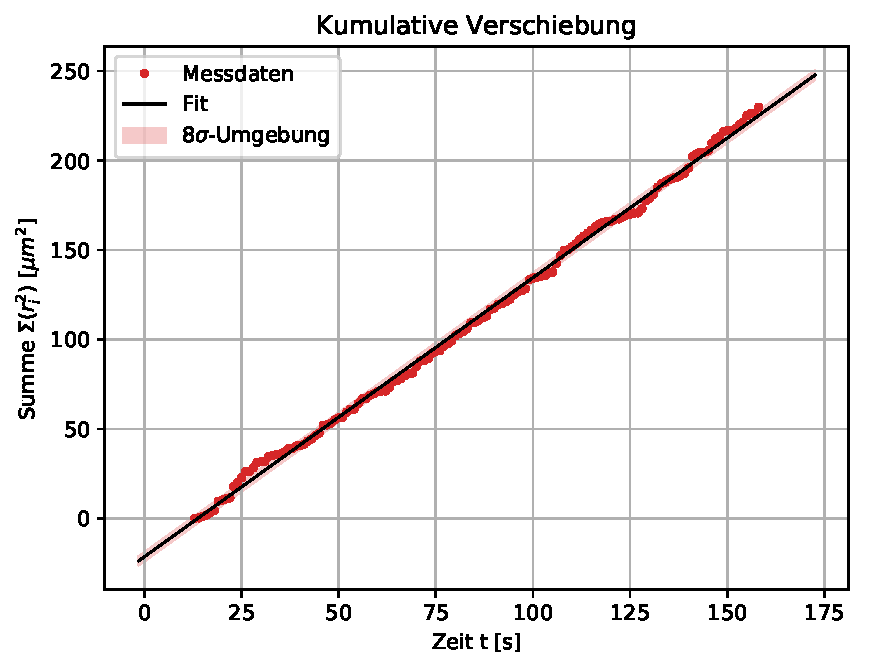
\includegraphics[width=0.8\textwidth]{223_Fig3.pdf}}{1}
  \end{annotate}
\caption{}
\label{fig:Fig3}
\end{figure}
\section{Auswertung}
Wir vergleichen die folgenden Messwerte und die definierte Naturkonstante selbst:
\begin{align*}
 k_{B,1} = &1.70(44)\times10^{-23}\:J\:K^{-1}\\
 k_{B,2} = &1.69(42)\times10^{-23}\:J\:K^{-1}\\
 k_B = &1.380649\times 10^{-23}\:J\:K^{-1}
\end{align*}
zuerst ist festzustellen, das unsere Methoden die Boltzmann-Konstante zu berechnen im Prinzip genau das gleiche Problem beschreiben. Sowohl die Länge entlang des Pfades (Kumulierte Verschiebung) als auch uch der Erwartete Entfernung zwische Start- und Endposition skalieren linear, sogar proportional mit der Zeit.
Egal für welche Rechnung man sich entscheidet wird, das Ergebnis vom diesem Versuch ist deutlich im 1-Sigma-Bereich des Literaturwerts. Das liegt hauptsächlich an dem relativ großen Fehlern:
\begin{align*}
 \frac{\Delta k_{B,1}}{k_{B,1}}\approx 39\% 
\end{align*}
\begin{align*}
 \frac{\Delta k_{B,2}}{k_{B,2}}\approx 40\% 
\end{align*}
Den signifikantesten Anteil am Fehler hat der Teilchenradius \(a\) mit
\begin{align*}
 \frac{\Delta a}{a}\approx 25\%
\end{align*}
D.h. um die Messung deutlich zu verfeinern müssen entweder größere Teilchen betrachtet werden und/oder eine feinere Messung von \(a\) gefunden werden (z.B. Kamera mit besserem Auflösungsvermögen). Unter anderem werden größere Teilchen sich aber langsamer bewegen, was andere Probleme bei der Versuchsdurchführung hat.

\section{Fazit}
Die Wahl verschiedener Parameter bei der Versuchsdurchführung (in diesem Fall z.B. Radius des Teilchens) ist sehr wichtig und kann, das Ergebnis und die Genauigkeit des Versuches stark beeinflussen. Statistische Fehler bleiben immer erhalten. Zusätzliche Parameter bei der Anpassung von Messdaten an ein theoretische Modell, können systematische Fehler korrigieren, wenn sie Begründet sind. Sie können aber auch die Ergebnisgenauigkeit fälschlicherweise reduzieren, wenn sie keinem experimentellen oder theoretischen Grund dienen.
Trotzdem haben wir mit diesem Versuch die Boltzmann-Konstante \(k_B\)  nur auf bis zu den Faktor 1.39 genau messen können und keiner der Messwerte weich mehr als um 1-Sigma von einander oder dem wahren Wert ab.
 \begin{align*}
 k_{B,1} = &1.70(44)\times10^{-23}\:J\:K^{-1}\\
 k_{B,2} = &1.69(42)\times10^{-23}\:J\:K^{-1}\\
 k_B = &1.380649\times 10^{-23}\:J\:K^{-1}
\end{align*}


\unboldmath
\end{document}
